%%%%%%%%%%%%%%%%%%%%%%%%%%%%%%%%%%%%%%%%%%%%%%%%%%%%%%%%%%%%%%%%%%%%%%
% Problem statement
\begin{statement}[
  problempoints=20,
  timelimit=1 sekunda,
  memorylimit=512 MiB,
]{Osijek}

\setlength\intextsep{-0.1cm}
\begin{wrapfigure}[6]{r}{0.22\textwidth}
\centering
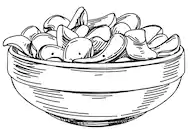
\includegraphics[width=0.22\textwidth]{img/chips.png}
\end{wrapfigure}

Morao je doći i taj dan. Lega, vatreni navijač Osijeka, navijač koji nikad
nije propustio nijednu Osijekovu prvenstvenu utakmicu, izgubio je dobar glas
i po preporuci liječnika ne smije na veliki derbi. Zato Lega, umjesto da je u
Gradskom Vrtu, sjedi ispred televizora i gleda utakmicu. Utjehu je pronašao u
kutiji čipsa. Dok je u kutiji bilo čipsa, Lega bi izvadio točno $K$ komada (ako
ih je nema toliko, izvadio bi koliko ima), pojeo ih i šaptom uzviknuo: ,,Ajmo
Bijelo-plavi!''.

Ako znamo da je u kutiji bilo $N$ komada čipsa, koliko je puta
Lega prošaputao navijački poklič?

%%%%%%%%%%%%%%%%%%%%%%%%%%%%%%%%%%%%%%%%%%%%%%%%%%%%%%%%%%%%%%%%%%%%%%
% Input
\subsection*{Ulazni podaci}
U prvom je retku cijeli broj $N$ $(0 \le N \le 100)$ iz teksta zadatka.\\
U drugom je retku prirodan broj $K$ $(1 \le K \le 100)$ iz teksta zadatka.

%%%%%%%%%%%%%%%%%%%%%%%%%%%%%%%%%%%%%%%%%%%%%%%%%%%%%%%%%%%%%%%%%%%%%%
% Output
\subsection*{Izlazni podaci}
U jedini redak ispišite traženi broj iz teksta zadatka

%%%%%%%%%%%%%%%%%%%%%%%%%%%%%%%%%%%%%%%%%%%%%%%%%%%%%%%%%%%%%%%%%%%%%%
% Scoring

%%%%%%%%%%%%%%%%%%%%%%%%%%%%%%%%%%%%%%%%%%%%%%%%%%%%%%%%%%%%%%%%%%%%%%
% Examples
\subsection*{Probni primjeri}
\begin{tabularx}{\textwidth}{X'X'X}
\sampleinputs{test/osijek.dummy.in.1}{test/osijek.dummy.out.1} &
\sampleinputs{test/osijek.dummy.in.2}{test/osijek.dummy.out.2} &
\sampleinputs{test/osijek.dummy.in.3}{test/osijek.dummy.out.3}
\end{tabularx}

\textbf{Pojašnjenje prvog probnog primjera:}
U kutiji je bilo $10$ komada čipsa. Lega je $5$ puta uzimao po $2$ komada i
uzvikivao navijački slogan.

%%%%%%%%%%%%%%%%%%%%%%%%%%%%%%%%%%%%%%%%%%%%%%%%%%%%%%%%%%%%%%%%%%%%%%
% We're done
\end{statement}

%%% Local Variables:
%%% mode: latex
%%% mode: flyspell
%%% ispell-local-dictionary: "croatian"
%%% TeX-master: "../hio.tex"
%%% End:
